\documentclass[12pt]{article}
\usepackage{design_ASC}
\hypersetup{
    colorlinks=true,
    linkcolor=cyan,
    filecolor=magenta,
    urlcolor=blue,}

% Subfigures
\usepackage{subfig}

\setlength\parindent{0pt} %% Do not touch this

%% -----------------------------
%% TITLE
%% -----------------------------
\title{Exercise List \#3} %% Assignment Title

\author{Victor F. Ferrari - RA 187890\\ %% Student name
vferrari@mpc.com.br\\
MO814A/MC937A - Topics in Computer Graphics\\ %% Code and course name
\textsc{Universidade Estadual de Campinas}
}

\date{\today} %% Change "\today" by another date manually
%% -----------------------------
%% -----------------------------

%% %%%%%%%%%%%%%%%%%%%%%%%%%
\begin{document}
\setlength{\droptitle}{-5em}    
%% %%%%%%%%%%%%%%%%%%%%%%%%%
\maketitle

% --------------------------
% Start here
% --------------------------

%%%%%%%%%%%%%%%
\section{Basic OpenGL}
%%%%%%%%%%%%%%%
{\bfseries Consider that you have a function \texttt{listOfVertices()} that generates a list of properly formatted vertices in OpenGL. Write the OpenGL code needed to draw a red polygon composed of these vertices.}

For the following code to work, the function \texttt{listOfVertices()} returns a float vector, containing the vertices in the correct format. No shaders were explicitly used. The coordinate (0, 0) is at the center of the screen.

\begin{Verbatim}[frame=single, fontsize = \footnotesize{}]
#include <iostream>
#include <vector>

#include <GL/glew.h>
#include <GLFW/glfw3.h>


int main(){

    // Initialize GLFW
    if( !glfwInit() ){
        std::cerr<<"Failed to initialize GLFW\n"<<std::endl;
        return -1;
    }

    // Open a window and create its OpenGL context
    GLFWwindow* window = glfwCreateWindow(600, 600, "Red Polygon", nullptr,nullptr);

    // Check if window was successfully created.
    if( window == nullptr ){
        std::cerr<<"Failed to open GLFW window"<<std::endl;
        glfwTerminate();
        return -1;
    }

    glfwMakeContextCurrent(window);

    // Initialize GLEW
    if (glewInit() != GLEW_OK){
        std::cerr<<"Failed to initialize GLEW"<<std::endl;
        glfwTerminate();
        return -1;
    }

    // Get Polygon
    std::vector<float> polygon = listOfVertices();

    GLuint vbo;
    GLuint vao = 0;

    // VBO
    // Generate and bind buffers (1)
    glGenBuffers(1, &vbo);
    glBindBuffer(GL_ARRAY_BUFFER, vbo);

    // Initialize buffer data.
    glBufferData(GL_ARRAY_BUFFER, polygon.size() * sizeof(float), polygon.data(), 
    	     GL_STATIC_DRAW);

    // VAO
    // Generate and bind vertex arrays (1).
    glGenVertexArrays(1, &vao);
    glBindVertexArray(vao);

    // Enable vertex attribute array.
    glEnableVertexAttribArray(0);

    // Define an array of generic vertex attribute data.
    glVertexAttribPointer(0, 3, GL_FLOAT, GL_FALSE, 0, nullptr);

    // Polygon Color : RED.
    glColor3f(1.f, 0.f, 0.f);

    while(glfwWindowShouldClose(window) == 0 ){

        // Draw polygon from the currently bound VAO.
        glDrawArrays(GL_POLYGON, 0, polygon.size());

        // Display
        glfwSwapBuffers(window);

        // Update other events (close button)
        glfwPollEvents();
    }

    // Close OpenGL window and terminate GLFW
    glfwTerminate();

    return 0;
}
\end{Verbatim}

% %%%%%%%%%%%%%%%%%%%%%%%%%%%%%%%
\section{Cohen-Sutherland Line Clipping}
% %%%%%%%%%%%%%%%%%%%%%%%%%%%%%%%
{\bfseries For each of the following line segments,
\begin{enumerate}
\item Determine the 2D Cohen-Sutherland codes for each vertex.
\item Determine whether this line is trivially rejected, trivially accepted, or clipped.
\item If the line segment must be clipped, compute the new endpoints.
\end{enumerate}
NOTE: Viewport size is 800x600, origin is at (0, 0) (bottom-left corner), points are defined in window coordinates.}

In the Cohen-Sutherland algorithm, each bit position indicates whether the point is inside or outside of a specific window edge. Each bit indicates one edge, as can be seen in Figure \ref{fig:cohen}.

\begin{figure}
    \centering
    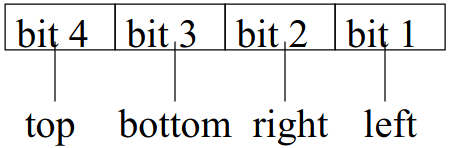
\includegraphics[width = 0.3\textwidth]{images/cohen.png}
    \caption{Cohen-Sutherland 2D Codes}
    \label{fig:cohen}
\end{figure}

\begin{itemize}
\item \textbf{ Line Segment 1: (-200, 700), (400, -300)}
\end{itemize}
	$c_0$: 1001, \hspace{1cm} $c_1$: 0100.

	Both vertices are outside the window, but $c_0 \land c_1 = 0$, so this line is not trivially rejected. Clipping is necessary. The line slope is $m=\frac{700-(-300)}{-200-400}=-\frac{5}{3}$, so the line equation for the segment is $3y = -5x + 1100$. The intersection with the top line, $y=600$, is at $x=-140$, so the new line segment is (-140, 600), (400, -300). Repeating the process...
    \bigbreak
 	$c_0$: 0001, \hspace{1cm} $c_1$: 0100.
    
	Both vertices are outside the window, but $c_0 \land c_1 = 0$, so this line is not trivially rejected. Clipping is necessary. The intersection with the left line, $x=0$, is at $y=\frac{1100}{3} \approx 367$, so the new line segment is (0, 367), (400, -300). Repeating the process...
	\bigbreak
	$c_0$: 0000, \hspace{1cm} $c_1$: 0100.
	
    One vertex is inside the window, and the other is outside the window, so this line is not trivially rejected or accepted ($c_0 \land c_1 = 0$). Clipping is necessary. The intersection with the bottom line, $y=0$, is at $x=200$, so the new line segment is (0, 367), (200, 0). Repeating the process...
	\bigbreak
	$c_0$: 0000, \hspace{1cm} $c_1$: 0000.
    
    Both vertices are inside the window, with code 0, so $c_0  \lor  c_1 = 0$. Therefore, this line is trivially accepted, and no clipping is necessary. Final segment: (0, 367), (200, 0).

    
\begin{itemize}
\item \textbf{ Line Segment 2: (100, 100), (400, 600)}
\end{itemize}
	$c_0$: 0000, \hspace{1cm} $c_1$: 0000.
    
    Both vertices are inside the window, with code 0, so $c_0  \lor  c_1 = 0$. Therefore, this line is trivially accepted, and no clipping is necessary. Final segment: (100, 100), (400, 600).

\begin{itemize}
\item \textbf{ Line Segment 3: (400, 300), (1000, 300)}
\end{itemize}
	$c_0$: 0000, \hspace{1cm} $c_1$: 0010.
	
    One vertex is inside the window, and the other is outside the window, so this line is not trivially rejected or accepted ($c_0 \land c_1 = 0$). Clipping is necessary. The line slope is $m=\frac{300-300}{400-1000}= 0$, so the line equation for the segment is $y = 300$. The intersection with the right line, $x=800$, is at $y=300$, so the new line segment is (400, 300), (800, 300). Repeating the process...
	\bigbreak
	$c_0$: 0000, \hspace{1cm} $c_1$: 0000.
    
    Both vertices are inside the window, with code 0, so $c_0  \lor  c_1 = 0$. Therefore, this line is trivially accepted, and no clipping is necessary. Final segment: (400, 300), (800, 300).

% %%%%%%%%%%%%%%%%
\section{Polygon Clipping}
% %%%%%%%%%%%%%%%%
\begin{enumerate}
\item  \textbf{Clip the polygon in figure \ref{fig:poly} using the Sutherland-Hodgman algorithm against the left, right, top, and bottom sides (in that order). NOTE: Just draw the output (approximately, but indicate vertices), don't need to show any math.}
\item \textbf{Clip the polygon in figure \ref{fig:poly} using the Weiler-Atherton algorithm. NOTE: Just draw the output (approximately, but indicate vertices), don't need to show any math.}
\end{enumerate}

The output of the Sutherland-Hodgman is one polygon, but has edges on top of the viewport, 	while the output of the Weiler-Atherton algorithm is composed of 3 different polygons. Every new vertex introduced has a different letter, following alphabetic order, from A to Z. If a letter is missing from the image, that vertex was introduced during the execution, and later discarded. The outputs can be seen in Figure \ref{fig:outputs}.

The output of Sutherland-Hodgman is in figure \ref{fig:hodgman} and the output of Weiler-Atherton is in figure \ref{fig:weiler}. The main difference, apart from the vertex labels, are the edges marked by the blue arrows.

\begin{figure}
    \centering
    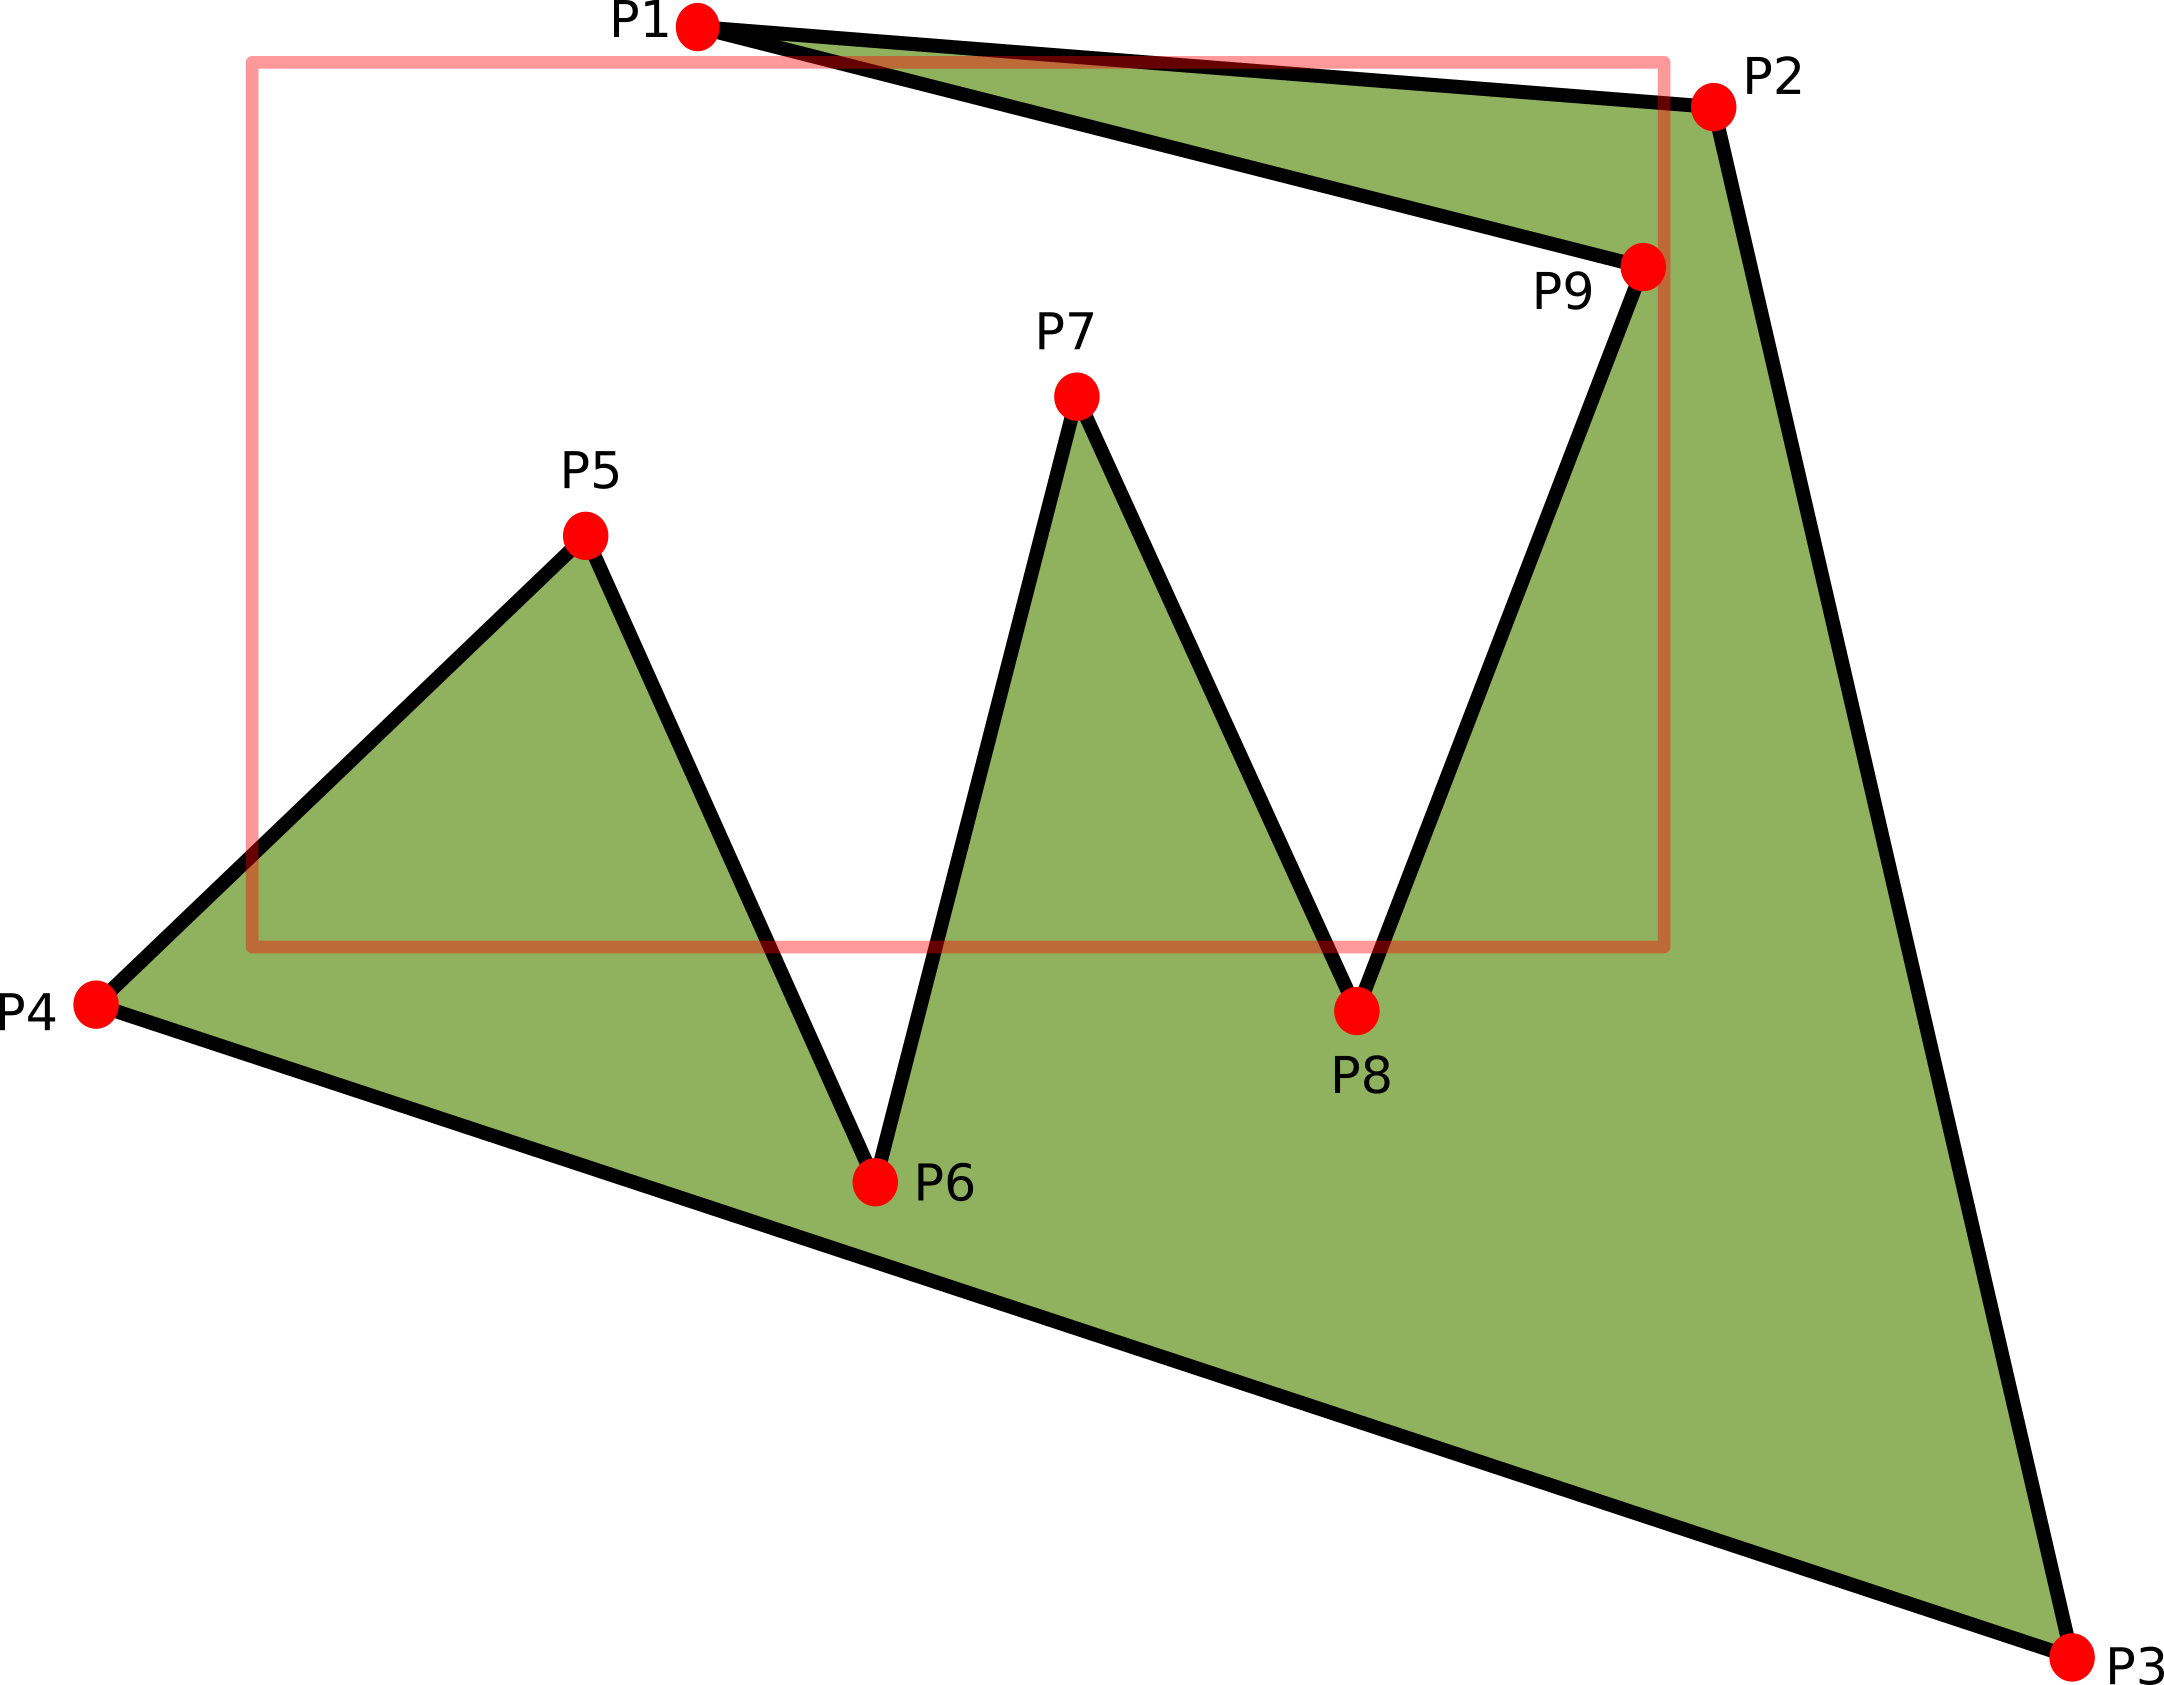
\includegraphics[width=0.5\textwidth]{images/poly.png}
    \caption{Polygon for clipping.}
    \label{fig:poly}
\end{figure}

\begin{figure}
    \centering
    \subfloat[Sutherland-Hodgman]{
    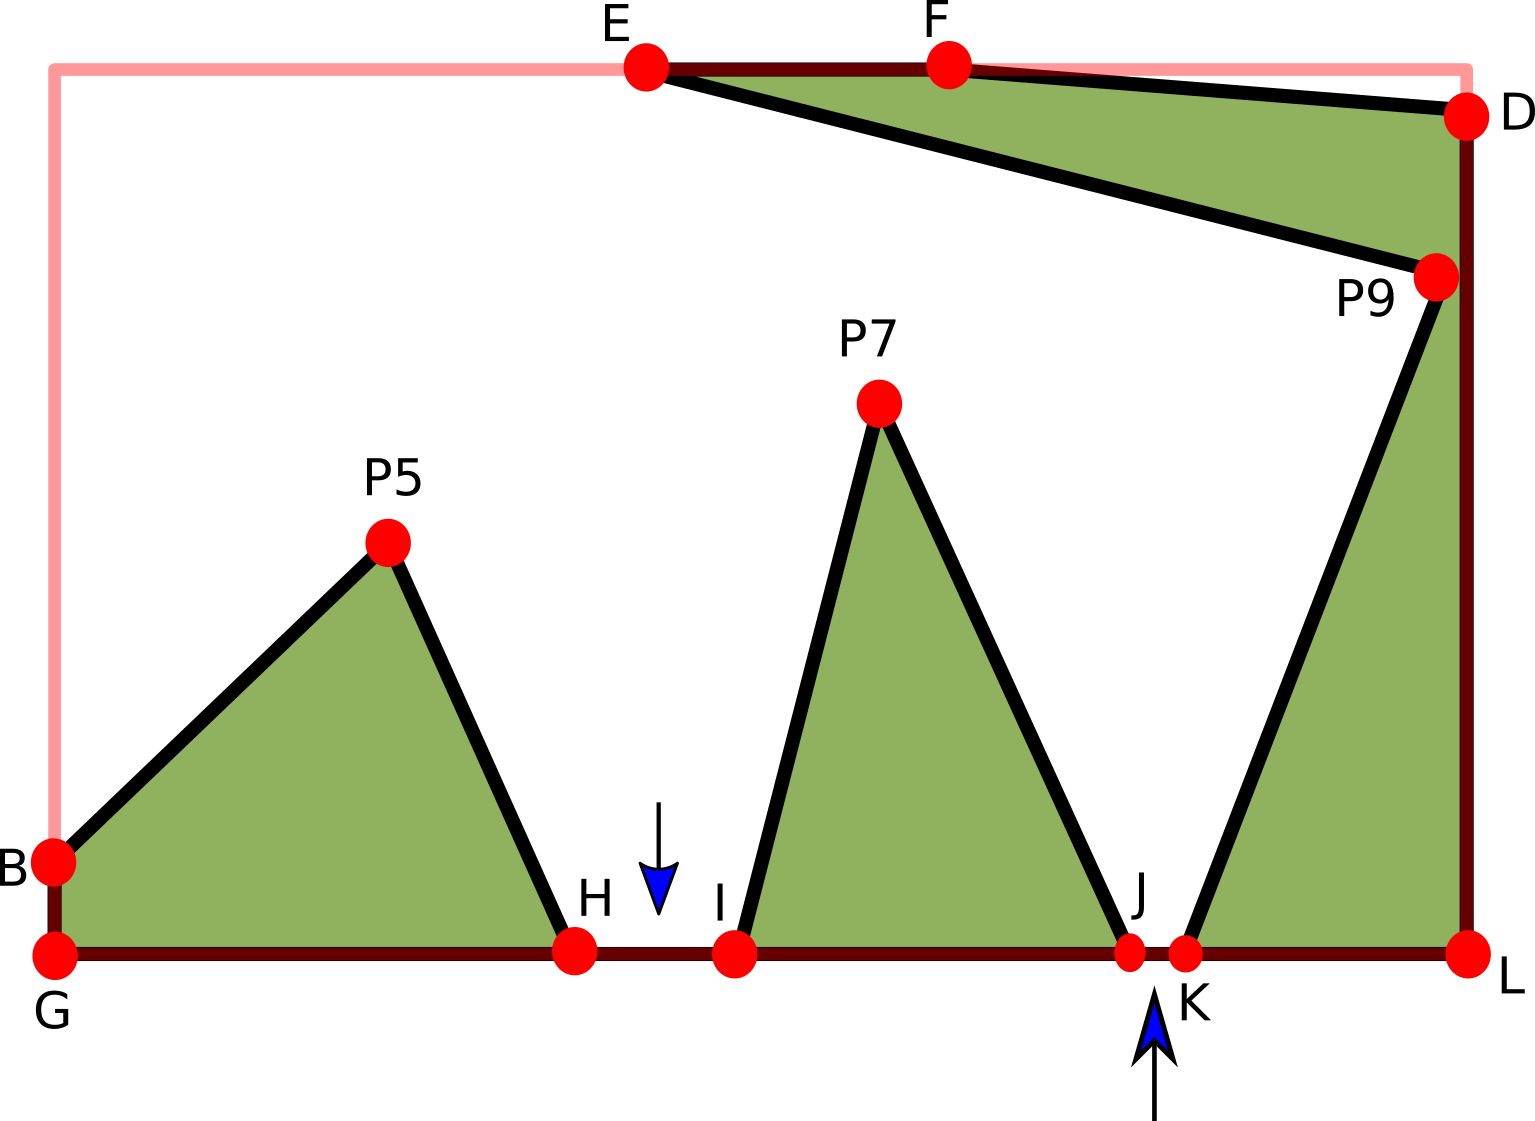
\includegraphics[width=0.5\textwidth]{images/hodgman.png}
    \label{fig:hodgman}
    }
    \qquad
    \subfloat[Weiler-Atherton]{
    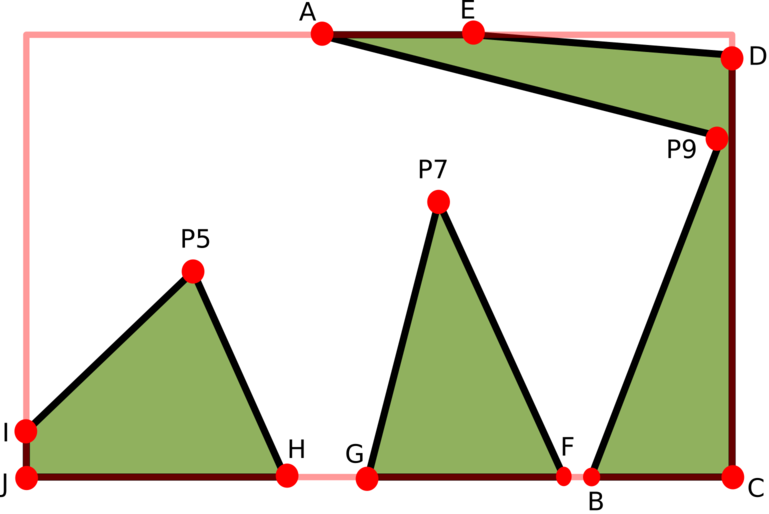
\includegraphics[width=0.5\textwidth]{images/weiler.png}
    \label{fig:weiler}
    }
    \caption{Outputs of clipping the polygon.}
    \label{fig:outputs}
\end{figure}

\end{document}